\chapter{Introduction - Project Context}
\pagestyle{headings}

Not long time ago, big data and the need for content analysis were idealistic, intangible concepts. However, recent developments in computer performance and the growing popularity of social media has enhanced the need for novel academic approaches in this field.

The biggest challenge with processing these huge amounts of data lies in its sheer volume. This is highly problematic in many different ways:

\begin{itemize}
 \item storing and managing data is costly and sometimes needs special structuring attention
\item irregularities across data streams often indicate the need for extra transformations
\item filtering out noise and the extraction of meaningful data from thousands of entries requires specialised algorithms, architectures and platforms which are either inaccessible or difficult to use by regular users
\end{itemize}

\section{Project context}

Social media platforms these days have a strong presence in "the Cloud", which allows more and more developers to solve the problem of storage space and scalability in a relatively easy way. The high adoption of platforms like Facebook, Twitter, Instagram and many others have resulted in the generation of hundreds of thousands of online documents, text and media alike. Such a deluge of information is highly applicable for business purposes, but in is often stuck as a "diamond in the rough". An array of new and exciting job titles has also appeared, such as "Social Media Marketer", "Social Media Manager", "Social Media Expert" and so on. Not only do they represent career alternatives for a new generation, but they are also still outliers for decision support software.

\subsection{Social Media and why people care about what it says}

While the concept of Social Media is not a new one to be precise, it is clearly just starting to engulf us. The spread of Social Media alongside the spread of worldwide Internet access, the emergence of specialised applications and the recent shift to mobile online presence are objective realities. Subjectively as well, people have become more engaged to consuming, creating and sharing content online, which is evident in newspaper sales drops, app sales increase, events "going viral" within groups and even the online presence of a political critical mass. Companies offer barter possibilities for a variety of bloggers and vloggers to push products to their followers (which is not only more effective\footnote{http://www.techrepublic.com/article/election-tech-why-social-media-is-more-powerful-than-advertising/}, but also cheaper).

No wonder social media has a stake in public decisions! But for the first time in decades, people's choices are also quite open and public. Which means that some parties can get clues about society's preferences by using public data available on platforms such as Facebook, Youtube and Twitter. Consider two basic use cases, which I will emphasise throughout the course of this thesis:

\begin{itemize}
\item What does social media say about X?
\item What does social media say about X vs. Y?
\end{itemize}

where X and Y can be public people, events, brands, companies etc. 

\subsection{Data Analysis tools today}

There are a number of current platforms for data analysis, in the large sense including chart generators, format converters and importers and data visualisation plug-ins of sorts. Crossing into the realm of powerful analysis applications, most of them are complex and confusing to non-engineers, examples including Tableau\footnote{https://public.tableau.com/s/}, RapidMiner\footnote{http://rapidminer.com} and WolframAlpha\footnote{http://www.wolframalpha.com}. Figure \ref{fig:tableau} shows Tableau's interface, which may seem quite intimidating.

\begin{figure}[ht]
    \centering
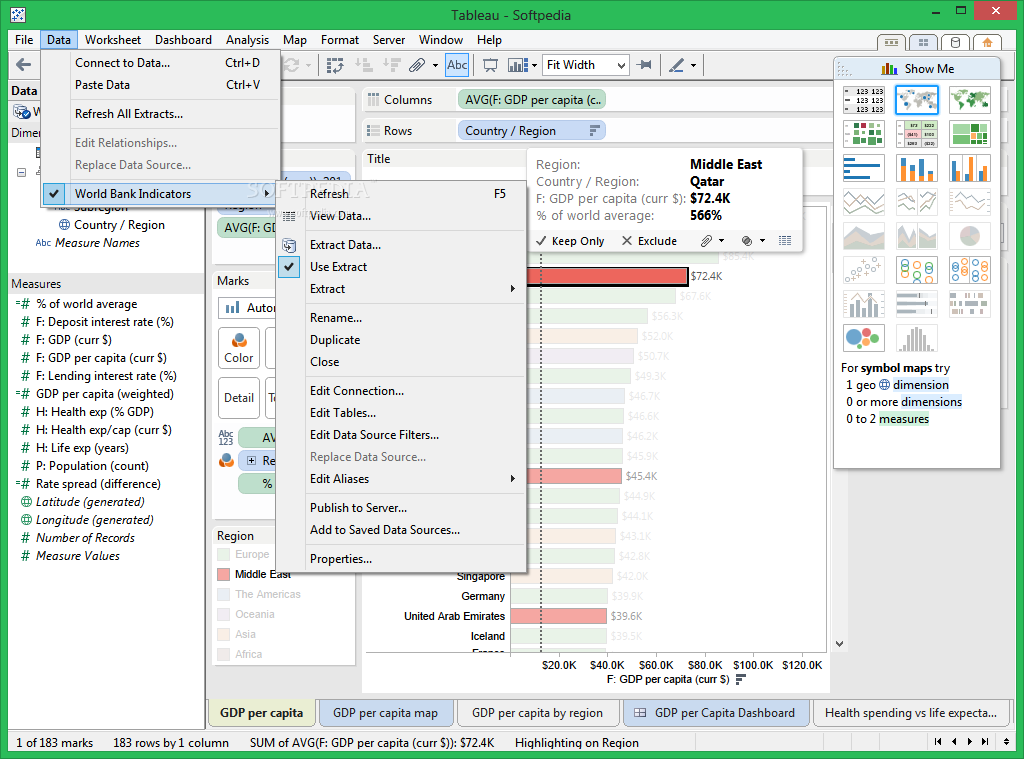
\includegraphics[width=0.7\columnwidth]{img/Tableau-Desktop_3.png}
    \caption{Tableau's interface}
    \label{fig:tableau}
\end{figure}

\subsection{Crossroads: Social Media in Business Intelligence}

The Computer Science field is very much branched nowadays in clearly-delimited subjects. But it is such a case where the large-scale processing capacities of data analytics should merge with approaches for computer-assisted business decisions. Consider that data analytics software often requires extensive training and a specialised knowledge, while most users desire only simple, straightforward functionalities for basic data analysis. One of Object Oriented Programming's fundamental principles is that of abstraction, in which end users need not (and should not) be aware of what is under the hood. Yet in data analytics, this is still the case on a 

The following Master's Thesis is the result of such an endeavour, to combine solid concepts from big data analysis, web application architecture and design, as well as enterprise software and economics for a better understanding of social media trends and opinions.

\subsection*{Thesis structure}
This document describes the general context, theoretical foundations and implementation details of a proof of concept application called "Approach for Twitter Harvesting, Enhancement, Normalisation \& Analysis" or, in short, ATHENA. Chapter 2 presents the objectives and requirements of our proposed system. Chapter 3 presents scientific approaches already validated by the community, some of which are generally similar to the entire ATHENA pipeline, while some are concerned with parts of the proposed implementation. Chapter 4 and 5 present a theoratical analysis and a detailed implementation of ATHENA respectively. Chapter 6 presents the testing and validation methods used as per ensuring application quality and usefulness. The final chapters contain technical instructions for installing the project, as well as the conclusions drawn from ATHENA's development endeavour.